\chapter{Authentication techniques and architectures}

\section{What is authentication}


\subsection*{Definitions of authentication}
There are three different definitions of \emph{authentication:}
\begin{itemize}
  \item \textbf{RGC-4949 (Internet security glossary)}:\\
        "the process of verifying a claim that a system entity or system
        resource has a certain attribute value"
  \item \textbf{\url{whatis.com}}:\\
        "the process of determining whether someone or something is
        who or what it is declared to be"
  \item \textbf{NIST IR 7298 (Glossary of Key Information Security Terms)}:\\
        "verifying the identity of a user, process, or device, often as a
        prerequisite to allowing access to resources in an information
        system"
\end{itemize}
The key aspects of these definitions  are that they define the authentication of an actor, meaning that \textbf{it could be not only a human being} (interacting via software running on hardware) \textbf{but also a software component or a hardware element} (interacting via software). The common shorthand for authentication is \texttt{authN} or \texttt{authC}, while \texttt{authZ} is used for authorization, \textit{which is different but related}.
% Maybe add a cross-reference to "different but related", idk to what yet


\subsection*{Authentication factors}
While authenticating an \emph{actor}, there are three categories of \textbf{authentication factors} that can be used:
\begin{itemize}
  \item \textbf{Knowledge}: authentication relies on something that \emph{only the user knows}, for example a static
        passphrase, code, or personal identification number.\\
        The associated risks involve the storage of this
        knowledge, how it can be demonstrated, and the way it is transmitted.
  \item \textbf{Ownership}: authentication relies on something that \emph{only the user possesses} (often called an
        "authenticator"), for example, a token, smart card, or smartphone.\\
         The associated risks can be related
        to the authenticator itself, such as the possibility of infection with malware, the potential for it to be
        manufactured in a country that imposes government control, or the risk of it being stolen, cloned, or
        used without the owner's authorization (e.g., forgetting an unlocked smartphone).
  \item \textbf{Inherence}: \emph{something the user is}, for example, a biometric characteristic (such as a fingerprint).\\
        The associated risks include counterfeiting and privacy concerns. Inherence factors pose a greater risk
        than the previous cases because, for example, a biometric characteristic \ul{cannot be
        replaced when compromised}. For this reason, inherence factors should be limited to very secure environments,
        typically used only for local authentication, as a mechanism to unlock a secret or a device.
\end{itemize}


\section{Digital authentication model (NIST SP800.63B)}

% Image from slide
% \begin{figure}[h]
%   \centering
%   \includegraphics[page = 6,trim = 1cm 2.1cm 1cm 3.8cm, clip, width = 0.50\textwidth]{\slides}
%    \caption*{General model for digital authentication as described in NIST SP800.63B}
% \end{figure}

\begin{figure}[h]
  \centering
  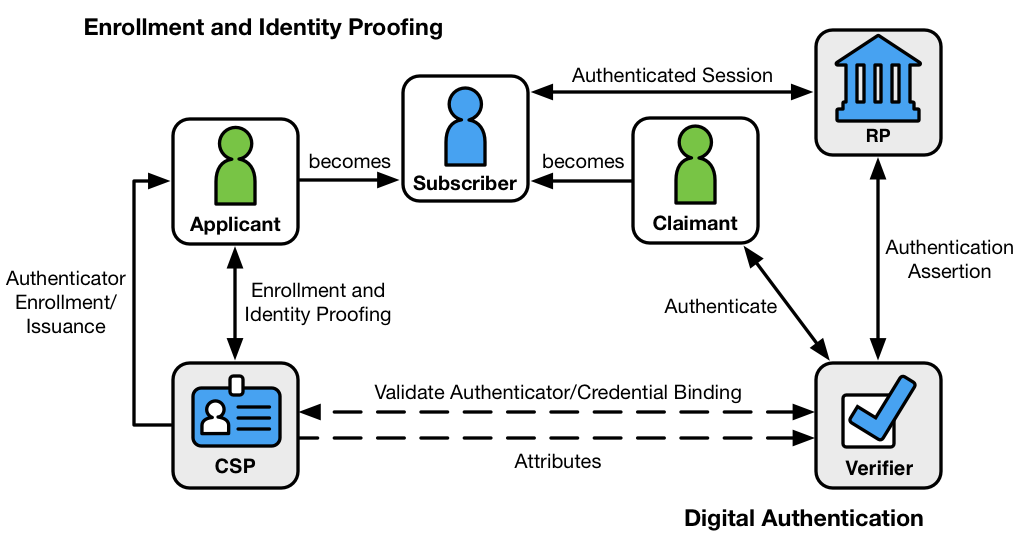
\includegraphics[width = 0.70\textwidth]{chapter3/NIST_sp800_63b.png}
  \caption*{General model for digital authentication as described in
  NIST SP800.63B}
\end{figure}

\begin{itemize}
  \item In this model, an actor who wants to use a system
  is called an \colorbox{LimeGreen}{\textbf{applicant}}: if it possesses an
  authenticator it can provide it to the \colorbox{Goldenrod}{\textit{CSP} (Credential Service Provider)}, or it can get one (for example, when a student is enrolled in Politecnico,
  he is given a smart card that works as an
  authenticator). The CSP is that component that will
  issue or enrol user credential and authenticator, and verify and store associated attributes.


  When this procedure is completed successfully, the actor becomes a \colorbox{Cyan}{\textbf{subscriber}}, which is an entity recorded in the authentication system.


  \item Later, when the actor wants to use some network service, typically the actor is called a \colorbox{LimeGreen}{\textbf{claimant}}, because they claim to be a valid user. Typically, an authentication protocol against a \colorbox{Goldenrod}{verifier} is run to verify this claim. When this process ends successfully, the actor becomes 
  \colorbox{Cyan}{\textbf{a subscriber}} \textbf{with an open authenticated session} with the \colorbox{Goldenrod}{relying party}, that will request and receive an authN assertion from the Verifier to assess user identity (and attributes).

  The relying party, which requests the actor to be authenticated, is the end application. The verifier may have communication with the CSP to validate the binding between the authenticator used in the authentication protocol and the credential claimed.
\end{itemize}

\subsubsection*{Recap}
\begin{itemize}
  \item \textbf{The credential binds an authenticator to the subscriber via an ID}: 
  \begin{itemize}
    \item for example, an X.509 certificate can be considered the credential, as it binds the identity and attributes written inside the certificate with the authenticator. In this case, the authenticator is the private key that the user controls.
  \end{itemize}
  \item \textbf{CSP (Credential Service Provider)}: 
  \begin{itemize}
    \item will issue or enrol user credential and authenticator
    \item verify and store associated attributes
  \end{itemize}
  \item \textbf{Verifier}:
  \begin{itemize}
    \item executes an authN protocol to verify possess of a valid
    authenticator and credential
  \end{itemize}
  \item \textbf{Relying party}:
  \begin{itemize}
    \item will request/receive an authN assertion from the Verifier to
    assess user identity (and attributes)
  \end{itemize}
\end{itemize}


These roles may be separate or collapsed together. 
Thinking about a \emph{Linux machine} used locally, the enrollment phase involves creating a new user with a username (the credential) and a password (the authenticator). In this scenario, the CSP is the operating system itself, and when a user wants to use a server on this machine, they need to perform login, which is the verifier. The relying party is any software running on that machine that uses the identity as proven by the login service of the operating system.


Another example is the use of Google Identity for different services, such as the Doodle Service to agree on a date. For Doodle, there is the option to use Google or Facebook Credentials. In this case, the relying party is Doodle, while the verifier (as well as the CSP) is Google or Facebook.


Another example is the use of Google Identity for different services, such as the Doodle Service to schedule an
appointment. For Doodle, there is an option to use Google or Facebook Credentials. In this case, the relying party
is Doodle, while the verifier (as well as the CSP) is Google or Facebook.


\section{Generic authentication protocol}

\begin{figure}[h]
  \centering
  \includegraphics[page = 8,trim = 0.4cm 3cm 0.4cm 5.5cm, clip, width = 0.55\textwidth]{\slides}
\end{figure}
Suppose that the user wants to access an application server (Relying Party). In this case, the server will include both the Relying Party and Verifier. 
The user has been identified with the User ID and has a secret associated with that User ID. 
The server's identifier contains a table with the User ID and the result of the function $f$ applied to the secret. Normally, the secret should never be stored in cleartext; of course, if the function $f$ is the identity function, it means you are storing the secret in cleartext, which is not recommended.

When the user wants to access the service, they receive an \textbf{authentication request}. Initially, they provide the \textbf{User ID}, and then the verifier asks for a \textbf{proof request}; the user replies with the \textbf{proof $ = F(S_{\mathrm{UID}})$}, which is the result of the computation with the function $F$ applied to the user's secret. 

In this scenario, several problems need to be addressed:
\begin{itemize}
  \item On the user side, how is the secret stored? How is the secret provided (e.g., if it is a password entered via a keyboard, a keylogger could disclose it)? Is the transmission of the proof secure? 
  \item On the server side, how are the secrets related to the user stored? When a proof is received, how is it verified to be the correct proof?
\end{itemize} 

\section{Passwords (reusable)}
\begin{figure}[h]
  \centering
  \includegraphics[page = 9,trim = 0.4cm 5cm 0.4cm 5.5cm, clip, width = 0.55\textwidth]{\slides}
\end{figure}


Imagine that the secret is a \textbf{reusable password} (meaning that it is always the same), and the user is identified by their User ID, with the secret being the password associated with that user. On the server side, there is a table containing usernames and passwords in plain text or a function $H$ computed over the password.

Once again, there will be an \textbf{authentication request}, followed by the user sending their \textbf{UID}. Then, a password request is made, and the user responds with \textbf{$P_{\mathrm{UID}}$}.

Assume the network is secure and focus on the verifier's side. The secret is the user's password, and the client creates and transmits the proof, typically using a function $F = I$, which is the identity function. The proof is the password sent in plain text, which is, of course, dangerous.

Now, looking at the server, when the server receives the password, it needs to check if it is correct or not:
\begin{enumerate}
  \item first case: if the function $f$ used to store the password is the \textbf{identity function} ($f = I$), then the proof is the password in cleartext. In this scenario, the server knows all the passwords in plain text, and verifying their correctness is simple. However, it is risky; if someone copies the database, they will gain access to all data.
  \item second case (\ul{the suggested one}): $f$ is not the identity function but a \textbf{one-way hash} (a digest of the password), and the server does not know the password in plain text but only the (unprotected) digest $H_{\mathrm{UID}}$. This means that access control is a bit more complex, as when the proof is received, the hash of the proof is computed and compared with the hash stored in the password database. If the database is stolen, the attacker will not have a copy of the plain-text passwords.
\end{enumerate}


\subsection*{Problems of reusable passwords}
Password-based authentication is usually convenient for the user, but only if they have to remember just one password, a reusable one. The current situation is unfortunate because in some applications, there is a need for several passwords that cannot be remembered by a person, so they would need to be stored on the user's side, which is a source of insecurity. The \textbf{disadvantages} of password-based authentication are:
The disadvantages of password-based authentication are:
\begin{itemize}
    \item The user-side password storage: it could be written on a post-it or on a client-side password manager (also called password wallet), that stores it encrypted typically using only one passphrase;
    \item Guessable passwords;
    \item Server-side password storage: the server must know the password in cleartext or an unprotected digest of it (dictionary attack);
    \item \textbf{Sniffing}: Password can be sniffed while it is sent across the network;
    \item \textbf{DB attacks}: There could be attacks to the password DB at the verifier (if DB contains plaintext or only obfuscated password);
    \item \textbf{Password guessing}: it is very dangerous if it can be done offline, for example against a list of password hashes;
    \item \textbf{Password enumeration}: if the password is limited in length or character type, or if authN protocol doesn't block 
    \item \textbf{Password duplication}: using the same password for different services, due to user password reuse. This could be a problem because if the user has the same password for a high-security service and for a weaker one, an attacker could discover it on the weaker system and have access to the high-security one;
    \item \textbf{Cryptography aging}: the solution adopted for verifying the secret should not be tied to a specific cryptographic algorithm, because it could be then difficult to adapt to the need for changing the algorithm used, due to new attacks and more computing power;
    \item \textbf{Password capture} via server spoofing and phishing;
    \item \textbf{MITM attacks}.
\end{itemize}


\subsection*{Password best practice}
\begin{itemize}
  \item Use a \textbf{mixture} of alphabetic characters (both uppercase and lowercase), digits, and special characters. Unfortunately, there are many systems that don't allow the use of special characters or impose limits on password length.
  \item Use a \textbf{long} password, preferably at least 8 characters in length.
  \item \textbf{Avoid using dictionary words}, as attackers often employ dictionaries from multiple languages.
  \item \textbf{Change your password frequently}. If the same password is kept for an extended period, attackers have more time to perform their computations. It's advisable to change your password at least once or twice a year to reduce the window of exposure.
  \item Whenever possible, \textbf{consider not using passwords}. However, this may be unavoidable unless biometric techniques are employed.
\end{itemize}

\subsection*{Storing passwords}
\subsubsection*{Storing passwords on the server-side}
\begin{itemize}
  \item Never store passwords in cleartext.
  \item If the password is \textbf{encrypted}, the server must have access to the encryption key in cleartext, which can be a security concern. To enhance security, it's recommended to \textbf{store a password digest}. However, be cautious of dictionary attacks that can be expedited by techniques such as \textbf{rainbow tables}. To mitigate these types of attacks, you can introduce an unpredictable element known as a "\textbf{salt}".
\end{itemize}


\subsubsection*{Storing password on the client-side}
\begin{itemize}
  \item Should be only in user's head;
  \item If passwords are a lot, use an encrypted file or a password wallet;
  \ifthenelse{\boolean{showNew}}{
  \item It's better use an encrypted file, or a "password wallet / manager".
  }{}
\end{itemize}

\subsubsection*{Storing passwords on the client-side}
\begin{itemize}
  \item Passwords should be memorized by the user.
  \item If there are numerous passwords to manage, consider using an encrypted file or a password wallet.
\end{itemize}



\subsection*{The "Dictionary" Attack}
\begin{figure}[h]
  \centering
  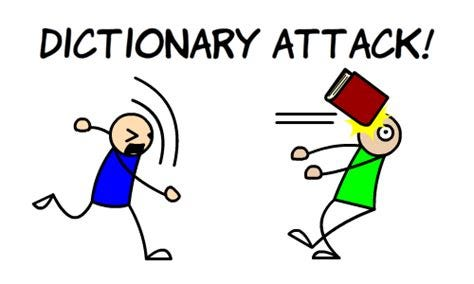
\includegraphics[width = 0.30\textwidth]{chapter3/dictionary_attack.jpg}
\end{figure}

If you store the plain hash of a password, dictionary attacks are possible. This is possible under two hypotheses:
\begin{enumerate}
  \item known hash algorithm;
  \item leakage of information, so that the attacker has a copy of the \textbf{password hash values}.
\end{enumerate}
Hashes are not invertible functions, but it is possible to make a \textbf{pre-computation}. Therefore, even if there is no copy of any password hash yet, it is possible to decide that it would be worthwhile to attack passwords stored as plain SHA-1 hashes in the future.

You must obtain a dictionary containing not only the Italian language but all possible languages. 
For each word in the dictionary, you compute the hash of the word and store it in a database paired with the corresponding word. 
By "word," we mean a potential passphrase, not a part of it. 
Typically, attackers have dictionaries extended to include words such as names of famous people.


The main hypothesis is that the user has chosen one of the words contained in the dictionary. The attack proceeds as follows:
\begin{enumerate}
  \item At some point, the attacker obtains a hash value due to a leakage.
  \item The attacker performs a simple \textbf{lookup} as follows: 
  \( w = \mathrm{lookup}(\mathrm{DB}, \mathrm{HP}) \), 
  where DB is the database
  and HP is the computed hash of a word in the database, if any of the hash passwords appears in any tuple.
  \item If the response is positive, the password is equal to that word. If not, the password is not from the dictionary.
\end{enumerate}

\textbf{Pre-computation} is the key because if you wait until you get a copy of the password hash, and only at that point you start computing all the possible hash values, it could be too late because the password could have changed.

\subsection*{Rainbow table}
A dictionary attack can be made faster and more effective by the \textbf{Rainbow table} technique. It is still a \textit{dictionary attack}, \ul{but it involves a trade-off between space and time}. Trying all possible passwords and computing the hash would be fast, but the result would be a huge database. If you have a complete database, the lookup would be fast, but fewer passwords are stored, and a bit more time is taken to compute the password if the corresponding hash is present. This is an improvement because \ul{it makes an exhaustive attack feasible for certain password sets}.

Imagine creating a rainbow table to attack a password that we know contains 12 digits. 
The exhaustive attack would require $10^{12}$ rows, which is a huge number of lines containing passwords and the corresponding hash values. 
A rainbow table could be used to reduce the number of rows in the database by a factor of 1000. In this way, we get a $10^9$ rows database, where each line represents 1000 passwords. To achieve that, we use the \textbf{reduction function}:
\[
r: h \Rightarrow p
\]
It is a function $r$ that takes as input a hash and creates one possibile password. Beware that this is NOT the inverse of the hash ($h^{-1}$), because the inverse of hash does not exist. It is just a mapping function that from a hash creates one of the possible passwords of the whole set.

\paragraph*{Pre-computing}
Then, the pre-computing is the following:

\begin{figure}[h]
  \centering
  \includegraphics[page = 15,trim = 1cm 2.5cm 7cm 13cm, clip, width = 0.55\textwidth]{\slides}
\end{figure}

\begin{enumerate}
  \item Select $10^9$ distinct passwords (the wanted size) called P
  \item For each of them initialize the computation starting from that specific password, and then iterate for 1000 times; each times the has of the current password is computed (called k) and then the reduction function is used to go from k to another possible password;
  \item At the end, the password P of the first cycle is stored in the database together with the last computation of the reduction function (called p).
  \item Then, the entry implicitly represents all the 1000 password tried. Not that there is no more has to be stored.
\end{enumerate}